\chapter{Grundlagen}
\label{chap:basics}
\todo[size=\small, inline]{Unbedingt besseren Namen für Kapitel "`Grundlagen"' finden!}%
\textbf{Hier kommt nur rein was ICH mache!}\\
An dieser Stelle soll zunächst ein Überblick über die in der vorliegenden Arbeit verwendeten Techniken gegeben werden. Diese beinhalten unter anderem Algorithmen der Computergrafik, welche Datenstrukturen benutzt werden und wie die Speicherverwaltung angesprochen wird.

\section{Datenstrukturen}
\label{sec:basics:datenstrukturen}
\textbf{Wofür und warum?!}\\
3D-Modelle aus CAD-Daten werden üblicherweise nach ihrer Funktion gruppiert. Das mag beim Entwurf solcher Systeme auch praktisch sein, beim ihrer Visualisierung kann dies jedoch zu Problemen führen. 
\todo[size=\small, inline]{Genaue Herkunft des Boeing-Modells finden!}%
Bei einem CAD-Modellen in der Größenordnung der Boeing 777 (ca. 350.000.000 Dreiecke) ist es wichtig, dass diese in eine geeignete räumliche Unterteilung überführt werden. Da ein Out-Of-Core-Renderer entwickelt wurde, findet ein ständiges Laden und Verwerfen von Teilmodellen statt. Je länger ein Renderer benötigt um herauszufinden, welche Teile des Modells er verwerfen kann und welche er als erstes Anfordern sollte, desto länger braucht er auch um ein Bild zu erstellen. In dieser Arbeit wurde als hierarchische räumliche Unterteilung ein Randomized Sampletree \ref{sec:basics:sampletree} und zum Vergleich ein Loose Octree gewählt.

\subsection{Loose Octree}
\label{sec:basics:octree}
\textbf{Warum ein Loose Octree?}\\
Um einen Octree \cite{RTR3} zu Erzeugen wird die gesamte Szene in eine minimale Boundingbox eingeschlossen. Rekursiv wird diese Box entlang der drei räumlichen Achsen in der Mitte geteilt, woraus sich jeweils acht gleich-große Boundingboxen ergeben. Dieser Vorgang wird so lange wiederholt bis ein Haltekriterium erfüllt ist. Im Falle der Boeing wurde festgelegt, dass nicht mehr als 5.000 Dreiecke in einer Box liegen dürfen und die maximale Tiefe des Baums wurde auf 14 beschränkt. Dies hat zur Folge, dass leere Boundingboxen nicht weiter aufgeteilt werden müssen. In Abbildung \ref{fig:basics:octree} ist ein Octree zu sehen.\\
Als Spezialfall wurde jedoch eine spezielle Form des Octrees verwendet: der Loose Octree. Dieser erweitert den Octree um eine weitere Box pro Knoten: die sogenannte Loosebox. Sie teilt sich ihr Zentrum mit der Octree-Boundingbox, besitzt aber doppelte Kantenlängen. Wird nun festgestellt, dass in einem Knoten mehr als 5.000 Dreiecke liegen, wird die größe der einzelnen Dreiecke anhand der Loosebox geprüft. Liegt ein Dreieck vollständig in der Loosebox mit seinem Zentrum in der eigentlichen Boundingbox des Knotens, kann es weiter nach unten gereicht werden. Ist die nicht der Fall, ist das Dreieck zu groß für den aktuellen Knoten und wird an den Vaterknoten gegeben.\\
Dies hat den Vorteil, dass große Dreiecke relativ weit oben im Baum zu liegen kommen. Je größer ein Dreieck ist, desto größer ist auch die Wahrscheinlichkeit, dass das Dreieck sichtbar ist und somit gezeichnet werden muss.

\begin{figure}
 \centering
  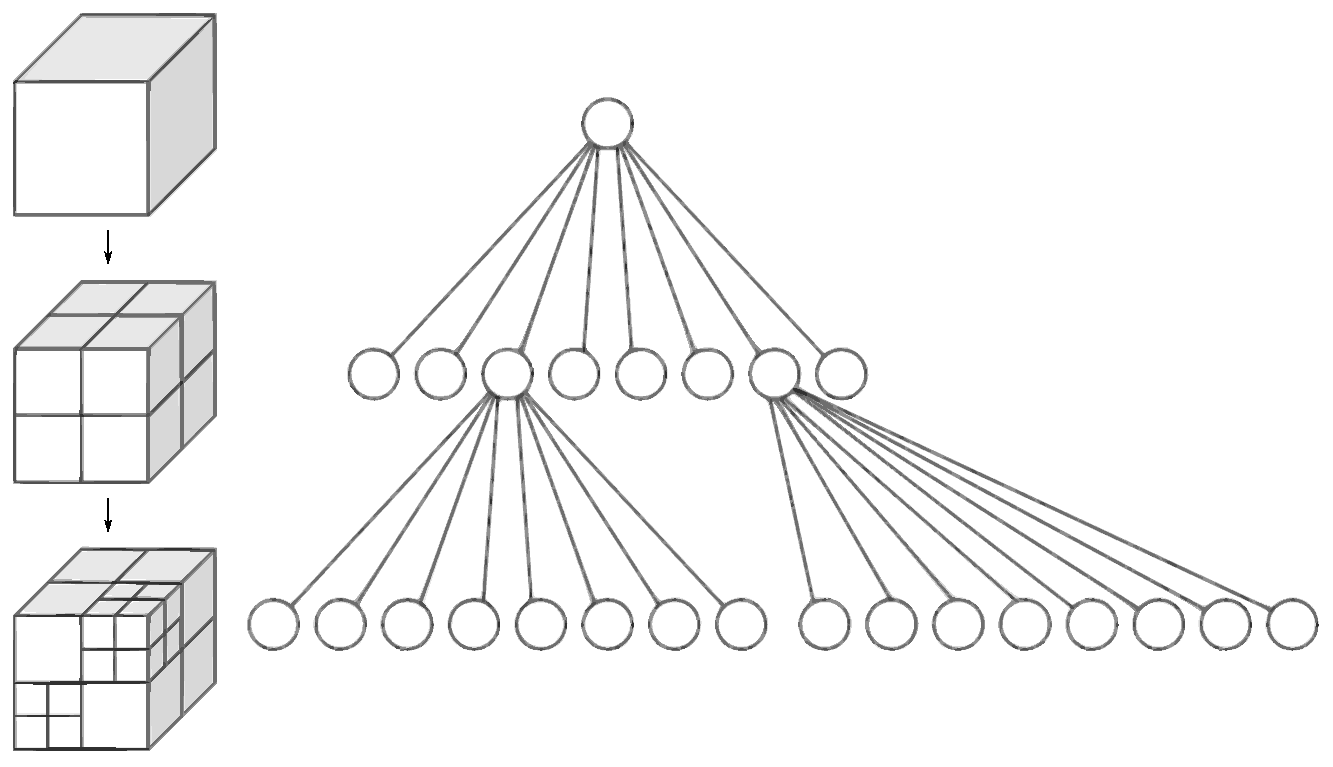
\includegraphics[scale=0.5]{images/octree.pdf}
 % octree.pdf: 640x368 pixel, 72dpi, 22.58x12.98 cm, bb=0 0 640 368
  \caption{Ein Octree der Tiefe 2. \textit{links: die räumliche Darstellung, rechts: die Baumdarstellung.}}
 \label{fig:basics:octree}
\end{figure}
\missingfigure{Bild zum Loose Octree}

\subsection{Randomized Sampletree}
\label{sec:basics:sampletree}
Als spezielle Ausprägung eines Loose Octrees gibt es den Randomized Sampletree \cite{klein}. Dieser unterschiedet sich von ein Octree darin, dass einzelne Dreiecke aus den tieferen Knoten nach oben gezogen wurden. Der Baum wird von unten nach oben durchlaufen. In jedem Knoten werden in Abhängigkeit der die Summe der Dreiecksflächen zufällig Dreiecke ausgewählt und in den Vaterknoten verschoben. Beim Rendern des Modells wird nun der Baum durchlaufen und falls die projizierte Größe der aktuellen Boundingbox die größe eines Pixel nicht überschreitet, wird die Baumtraversierung an dieser Stelle abgebrochen. Dadurch ergeben sich natürlich Darstellungsfehler. 
\todo[size=\small, inline]{Sampletree ausformulieren}%
Die zufällig nach oben verschobenen Dreiecke dienen als hinreichende Approximation. 
\missingfigure{Bild zum Randomized Sampletree}


\section{Computergrafik}
\label{sec:basics:computergrafik}
\todo[size=\small, inline, color=magenta]{Kapitel: Computergrafik}
Da Arbeitsspeicher in der Regel größer ist als der Speicher einer Grafikkarte, werden nicht alle geometrischen Objeke auf der Grafikkarte belassen. Wenn angeforderte Objekte bei einem Renderer eintreffen, werden die zunächst gar nicht an die Grafikkarte geschickt. Erst nach weiteren Tests, ob das Objekt immer noch sichtbar ist, findet der transfer zur GPU statt. Dort verbleiben sie dann, bis sie irgendwann aus platz- oder sichbarkeitsgründen verdrängt werden (siehe auch \ref{sec:basics:caching}). Um dies möglichst effizient umsetzen zu können werden Vertexbuffer Objects  (VBOs) genutzt. Die Idee ist dabei, dass Modelldaten, bestehend aus Vertices und Vertex-Normalen, in einem zusammenhängenden Speicherblock abgelegt werden. Ein Vertex besteht aus einer xyz-Koordinate und einer Vertex-Normalen. Der Zugriff auf Dreiecke erfolgt dann mittels einer Index-Liste, bei der immer drei Indices ein Dreieck ergeben. Alle Dreiecke eines Octree-Knotens wurden zu einem Vertexbuffer-Objekt zusammen gefasst (siehe \ref{sec:basics:octree}), da Geometrie innerhalb eines Knotens nicht weiter unterteilt wird. In Form von VBOs kann recht einfach entsprechender Platz im Grafik-RAM reserviert und die Daten in den Speicher geladen werden.\\
Im Gegensatz dazu verbleiben bei Vertex-Arrays alle Daten im Arbeitsspeicher des Rechners und werden für jeden Zeichenaufruf zur Grafikkarte übertragen. Vertex-Arrays bieten sich an, wenn Objekte nur einmal gezeichnet und dann verworfen werden. Von daher kommen sie nur auf den Datenknoten (siehe \ref{sec:impl:netzwerkarchitektur}) zum Einsatz, da diese ein getestetes Objekt nur in ihren Tiefenbuffer rendern und dann wieder verwerfen. Bei VBOs wäre der Overhead der Datenübertragung und der anschließenden Deallokation zu groß für eine einmalige Verwendung.
\begin{itemize}
 \item CgShader
 \begin{itemize}
  \item Beleuchtung -> Phong-Beleuchtungsmodell \cite{cgtutorial}
  \item Farben: Da bei CAD-Modellen Farben oft ein Hinweis auf den Produktionsort geben, ist die Anzahl der Fraben beschränkt. Natürlich könnte man jedem Vertex eine Farbe zuordnen. Dies hätte jedoch zur Folge dass bei jedem Vertex die Farbe neu gesetzt werden muss, unabhängig davon, ob diese Farbe bereits gesetzt ist, oder nicht. Das würde jedesmal die Grafik-Pipeline unterbrechen undes wäre mit Geschwindigkeitseinbußen zu rechen. Deshalb wurden die Farben der Boeing, 32 an der Zahl, in einer 1D-Textur codiert und die Texturkoordinate wurde als vierte Komponente an den Vertex gehängt. Wird nun ein Vertex gezeichnet, ersetzt der Vertex-Shader die harmonische Komponente wieder mit 1 und gibt die Textur-Koordinate an den Fragment-Shader weiter. Letzterer muss ohnehin eine Farbe schreiben, weshalb man diese kurzerhand aus der Textur ausliest.
  \missingfigure{Bild zur Textur mit den Farben und Texturkoordinaten-Range}
 \end{itemize}

\end{itemize}

\section{Approximation}
\label{sec:basics:approximation}
\todo[size=\small, inline, color=blue!40]{Kapitel: Approximation}
Approximationen in der Computergrafik haben oft  Zurfolge, dass die Bildqualität verringert wird. Sei es weil Objekte in niedrigeren Auflösungen
\begin{itemize}
 \item Teile können weggelassen werden
 \item Tiefenbuffer Update nur alle paar Frames
\end{itemize}

\section{Algorithmen}
\label{sec:basics:algorithmen}
\todo[size=\small, inline, color=blue!40]{Kapitel: Algorithmen}
\begin{itemize}
 \item Occlusion Culling \cite{RTR3}
 \item Frustum Culling \cite{RTR3}
 \item c-Collision Protokoll zur Lastbalancierung im Netzwerk
 \item c-Collision?: \cite{DBLP:conf/arcs/RehbergS99}: \textit{Almost optimal schedules with a simple protocol}
 \item adpative collision / c-Load, gewichtet: \cite{ccol2}: \textit{Allocating weighted jobs in parallel}
 \item c-Collision Basics: \cite{ccol3}: \textit{Parallel Balanced Allocations}
 \begin{itemize}
  \item $m$ Bälle in $n$ Körbe
 \end{itemize}
\todo[size=\small, inline]{c-Collisionprotokoll-Erklärung!}%
 \begin{itemize}
  \item auch bälle in Körbe aber diesmal haben die Bälle Gewichte
 \end{itemize}

\end{itemize}

\subsection{Caching}
\label{sec:basics:caching}
\todo[size=\small, inline, color=blue!40]{Kapitel: Caching}
\begin{itemize}
 \item wird über Algos gefüllt
\end{itemize}

\subsection{Speichermanagement}
\label{sec:basics:speichermanagement}
\todo[size=\small, inline, color=blue!40]{Kapitel: Speichermanagement}
\begin{itemize}
 \item nicht jeder braucht alles -> Kacheln
 \item Gewichtung über die Anzahl der Dreiecke pro Request
\end{itemize}
